% \section*{Tricks of the trade}
\subsection*{Matrix Things}
\textbf{SVD:} Suppose $\vM$ is a $m \cross n$ matrix whose entries are real or complex numbers. There exists a factorization, called a SVD of $\vM$, of the form
$ \mathbf {M} =\mathbf {U} {\boldsymbol {\Sigma }}\mathbf {V} ^{*}$
where \textbf{1)} $\vU$ is an $m \cross m$ unitary matrix over $K$ (if $K = \mathbb {R}$ , unitary matrices are orthogonal matrices), \textbf{2)} $\boldsymbol {\Sigma }$ is a diagonal $m \cross n$ matrix with non-negative real numbers on the diagonal (singular values), \textbf{3)} $\vV$ is an $n \cross n$ unitary matrix over $K$, and \textbf{4) }$\vV∗$ is the conjugate transpose of $\vV$.
A common convention is to list the singular values in descending order.\\
% \textbf{Diagonalization}\\
\textbf{Matrix calculus}\\
\tab$(\vA+\vB)'=\vA'+\vB'$, \tab$(\vA\vB\vC)'=\vA'\vB\vC+\vA\vB'\vC+\vA\vB\vC'$,\\
\tab$(\vA^n)'=\vA'\vA^{n-1}+\vA\vA'\vA^{n-2}+\ldots+\vA^{n-1}\vA'$,\\
\tab$(\vA\inv)'=-\vA\inv\vA'\vA\inv$, $(\det(\vA))'=\Tr(\vA'\vA)$,\\
\tab$(\vA\vx)'=\vA\T$, $(\vx\T\vA)'=\vA$, $(\vx\T\vx)'=2\vx$, \tab$(\vx\T\vA\vx)'=\vA\vx+\vA\T\vx$
% \textbf{Matrix math}\\
\tab$(\vA\vB)\T=\vB\T\vA\T$\\
$\mathbf{A}^{-1} = \begin{bmatrix}
a & b \\ c & d \\ 
\end{bmatrix}^{-1} =
\frac{1}{\det \mathbf{A}} \begin{bmatrix}
\,\,\,d & \!\!-b \\ -c & \,a \\ 
\end{bmatrix} =
\frac{1}{ad - bc} \begin{bmatrix}
\,\,\,d & \!\!-b \\ -c & \,a \\ 
\end{bmatrix}$


  $|A| = \begin{vmatrix} a & b & c \\ d & e & f \\ g & h & i \end{vmatrix}
    %  &= a\,\begin{vmatrix} \Box & \Box & \Box \\ \Box & e & f \\ \Box & h & i \end{vmatrix} - 
    %     b\,\begin{vmatrix} \Box & \Box & \Box \\ d & \Box & f \\ g & \Box & i \end{vmatrix} + 
    %     c\,\begin{vmatrix} \Box & \Box & \Box \\ d & e & \Box \\ g & h & \Box \end{vmatrix} \\[3pt]
     &= a\,\begin{vmatrix} e & f \\ h & i \end{vmatrix} - 
        b\,\begin{vmatrix} d & f \\ g & i \end{vmatrix} + 
        c\,\begin{vmatrix} d & e \\ g & h \end{vmatrix}$
    %  $&= aei + bfg + cdh - ceg - bdi - afh.$


\textbf{Trace identities and differentiation rules:}\\
$\vv^\top\vw = \sum\limits_i v_iw_i=\Tr(\vA+\vB) \quad \Tr(\vA+\vB)=\Tr(\vA)+\Tr(\vB)$\\
$\vE\Tr(\vX)=\Tr\vE[\vX]$
$\quad \nabla_\vA\Tr(\vA\vA^\top)=2\vA, \quad \nabla_\vA\Tr(\vA\vB)=\vB^\top$

\textbf{Definiteness of a matrix}:

\tab$\vA$ is positive definite if $\vx\T\vA\vx > 0,\>\> \forall \vx\neq0$
\tab$\vA$ is indefinite if it contains positive and negative eigenvalues.

\textbf{Finding Eigenvalues}:
$\det(\vA - \lambda \vI)=0$ and find values of $\lambda$. To get eigenvector for $\lambda_i$, plug $\lambda_i$ into $(\vA - \lambda_i \vI)\vv = 0$ and solve.\\
Roots of quadratic polynomial: 
$x=\frac{-b\pm\sqrt{b^2-4ac}}{2a}$

\subsection*{General Math}
\textbf{Derivative rules}\\
$\tan(x)\xrightarrow{}\sec^2(x),\>a^x\xrightarrow{}\ln(a)a^x,\>f/g\xrightarrow{}(f'g-g'f)/g^2$



\textbf{Sigmoid Derivative}: $\dv{\sigma(x)}{x} = \sigma(x)(1-\sigma(x))$\\

\textbf{Hessian:} when taking it, keep in mind that the second variable w.r.t which you take the the second partial derivative is what stays fixed per row.

\textbf{Integration by parts}: $\int u\>dv=uv - \int v\>du$\\
   $\int_a^b u(x) v'(x) \, dx 
   &= [u(x) v(x)]_a^b - \int_a^b u'(x) v(x) dx\\
   &= u(b) v(b) - u(a) v(a) - \int_a^b u'(x) v(x) \, dx $

\textbf{Integration by Substitution:}
$\int f(g(x))g'(x) dx \rightarrow \int f(u) du$

\textbf{Fundamental Theorem of Calculus}: $f(y)-f(x)=\int^y_x\nabla f(\tau) d\tau$

\textbf{Mean}: $\mathbb{E}\lbrack f(x) \rbrack = \int_x x\>f(x)\>dx$ \textbf{Variance:} $\mathbb{E}\lbrack f(x) \rbrack = \mathbb{E} \lbrack f(x)^2\rbrack - \mathbb{E} \lbrack f(x) \rbrack^2$

\textbf{Convexity of $f$ implies}: $f(y)\geq f(x)+\nabla f(x)\T (y-x), \forall (x,y) \in \R^{d\times d}$

\textbf{Jensen's inequality:} Let $(\Omega, A, \mu)$ be a probability space, such that $\mu(\Omega)= 1$. If $g$ is a real-valued function that is $\mu$-integrable, and if $\varphi$ is a convex function on the real line, then:
$\varphi\left(\int_\Omega g\, d\mu\right) \le \int_\Omega \varphi \circ g\, d\mu.$

\textbf{Cauchy-Schwarz}: $\lvert \langle \vu ,\vv \rangle\rvert^2\leq\langle \vu,\vu\rangle\cdot\langle\vv,\vv\rangle$

% $\xrightarrow{} \lvert\langle\vu,\vv\rangle\rvert\leq\lVert\vu,\vv\rVert $.

\textbf{Taylor Expansion}
\tab$f(x)=\sum\limits^\infty_{n=0}\frac{f^{(n)}(x_0)}{n!}(x-x_0)^n$ (exp. around $x_0$).

\tab$f(\vw)\approx f(\bar{\vw})+(\vw-\bar{\vw})\T\nabla f(\bar{\vw})+\frac{1}{2}(\vw-\bar{\vw})\T H (\vw-\bar{\vw})$

\textbf{Taylor-Lagrange}:
$f(x)=\sum\limits^n_{k=0}\frac{f^{(k)}(x_0)}{k!}(x-x_0)^k+\int\limits^x_{x_0}\frac{f^{(n+1)}(t)}{n!}(x-t)^n dt$.

\textbf{Taylor expansion with Lagrange remainder:}\\
$f(x)=\sum\limits^n_{k=0}\frac{f^{(k)}(x_0)}{k!}(x-x_0)^k+\frac{f^{(n+1)}(x_0+\theta(x-x_0))}{(n+1)!}(x-x_0)^{n+1}, \theta\in(0,1)$

\textbf{KL divergence}: $D_\text{KL}(P||Q)=-\sum_i P(i) \log \frac{Q(i)}{P(i)}= \sum_{x} P(x) \log\left(\frac{P(x)}{Q(x)}\right)$

% \textbf{Eigenvalues and vectors}: $H\vu_i=\lambda_i\vu_i$\\
% Eigenvectors are orthonormal (for real, symmetric): $\vu_i\T\vu_j=\delta_{ij}$

\textbf{Log Likelihood:} $\log\Pi^N_n p(t_n|x_n)=\log\Pi^N_n p(t_n=1|x_n)^{t_n} p(t_n=0|x_n)^{1-t_n}=\sum^N_n t_n \log p(t_n|x_n) + (1-t_n) \log (1-p(t_n|x_n))$

\tab put minus in front to get cross-entropy loss.

\textbf{Probability Names}: $P(Y|X)\xrightarrow{}$ likelihood, $P(X|Y)\xrightarrow{}$ posterior, $P(X)\xrightarrow{}$ prior, $P(Y)\xrightarrow{}$ evidence. Posterior = (likelihood * prior)/evidence

\textbf{Set Theory}
Compact = closed and bounded\\
$f\in\cC^{n+1}(\lbrack a,b\rbrack,\R)$: diff. $n+1$ times and is a mapping from $\lbrack a,b\rbrack$ to $\R$

\textbf{Newton's Method}: $\theta(t+1)=\theta(t)-\!\!\!\!\!\underbrace{(\nabla^2\cR)\inv}_\text{inverse Hessian}\!\!\!\!\!\nabla\cR\bigr|_{\theta=\theta(t)}$

\textbf{Sylvester's criterion}: necessary and sufficient criterion to determine whether a Hermitian matrix is positive-definite. All upper left corner matrices have to have a positive determinant.
% \href{https://en.wikipedia.org/wiki/Sylvester\%27s_criterion}{Aqui!}

% A differentiable function of one variable is convex on an interval if and only if the function lies above all of its tangents:
% $f(y)\geq f(x)+\nabla f(x)^T(y-x)$

\textbf{Weierstrass theorem:} If f is a given  continuous  function for $a\leq x \leq b$ and if $\epsilon$ is an arbitrary positive quantity, it is possible to construct an approximating polynomial $P(x)$ such that: $|f(x)-P(x)|\leq \epsilon, \quad a\leq x\leq b$

\subsection*{Misc. Deep Learning}
\subsubsection*{Loss Functions}
\textbf{L1-norm loss}: least absolute deviations (LAD), least absolute errors (LAE) 

\tab $L=\sum^n_{i=1} \lvert y_i - f(x_i) \rvert$

\textbf{L2-norm loss}: least-squared errors (LSE)

\tab $L=\sum^n_{i=1} \lVert y_i - f(x_i) \rVert^2$

\textbf{L2-regularized}:

\tab $L(x;\theta)=\sum^n_{i=1} \lVert y_i - f(x_i;\theta) \rVert^2 + \lambda\sum_{ij}\theta_{ji}^2$

\textbf{Mean Squared Error}: MSE

\tab $L=\sum^n_{i=1} \lVert y_i - f(x_i) \rVert^2 / n$

\textbf{Cross-Entropy Loss}: log loss

$L=-\log\Pi^N_n p(t_n|x_n)=-\log\Pi^N_n p(t_n=1|x_n)^{t_n} p(t_n=0|x_n)^{1-t_n}=-\bigr(\sum^N_n t_n \log p(t_n|x_n) + (1-t_n) \log (1-p(t_n|x_n))\bigr)$



\section*{Examples}
\subsection*{Ex4 P2: Approximate Hessian for feed-forward NN}
\textbf{Setup}: $a_j=\sum\limits_i w_{ji}z_i$, where $z_i$ is the activation of a unit that sends a connection to unit $j$, and $w_{ji}$ is the weight associated with that connection. Let $h$ be a nonlinear activation function, then $z_i=h(a_i)$. Evaluate second derivatives of the loss, $\frac{\partial^2 L}{\partial w_{ji} \partial w_{lk}}$. Recall the loss function decomposes over samples from the dataset as $L(\cdot)=\sum_n L_n(\cdot)$

\textbf{Compute $\frac{\partial L_n}{\partial w^2_{ij}}$ as a function of $z^2_i$.}\\

\tab$\frac{\partial L_n}{\partial w^2_{ij}}=\frac{\partial}{\partial w_{ji}}\cdot \frac{\partial L_n}{\partial w_{ji}}=\frac{\partial}{\partial w_{ji}}(\frac{\partial L_n}{\partial a_j}\cdot\frac{\partial a_j}{\partial w_{ji}})=\frac{\partial}{\partial w_{ji}}(\frac{\partial L_n}{\partial a_j}\cdot z_i)$\\

\tab Used: $\pdv{a_j}{w_{ji}}=\pdv{\sum_i w_{ji}z_i}{w_{ji}}=z_i$ for one specific $i$. Apply product rule:

\tab$\pdv{}{w_{ji}} (\pdv{L_n}{a_j}\cdot z_i)=\pdv{}{w_{ji}} (\pdv{L_n}{a_j})\cdot z_i+\pdv{L_n}{a_j}\pdv{z_i}{w_{ji}}$. (and $\pdv{z_i}{w_{ji}}=0$ since output of $i$ doesn't depend on $w_{ji}$).

\tab $\pdv{}{w_{ji}} ( \pdv{L_n}{a_j} )\cdot z_i=\pdv{}{w_{ji}} (\pdv{L_n}{w_{ji}})\cdot z_i=\pdv{}{a_j} (\pdv{L_n}{a_j}\pdv{a_j}{w_{ji}})\cdot z_i=\pdv[2]{L_n}{a_j}\cdot z_i^2$

\textbf{Show that:} $\frac{\partial^2 L_n}{\partial a_j^2}=h'(a_j)^2\sum\limits_k\sum\limits_{k'} w_{kj}w_{k'j}\frac{\partial^2 L_n}{\partial a_k \partial a_{k'}}+h''(a_j)\sum\limits_k w_{kj}\frac{\partial L_n}{\partial a_k}$

\tab use (by chain rule): $\pdv{L_n}{a_j} = \sum_k \pdv{L_n}{a_k} \cdot \pdv{a_k}{a_j}$\\
\tab For one specific $k$: $\pdv{a_k}{a_j} = \pdv{\sum_i w_{ki} z_i}{a_j} = \pdv{w_{kj} z_j}{a_j} = h'(a_j) w_{kj}$\\

\tab$\pdv[2]{L_n}{a_z} = \pdv{}{a_j} ( \pdv{L_n}{a_j} ) = \pdv{}{a_j} \bigr( h'(a_j) \sum_k w_{kj} \pdv{L_n}{a_k} \bigr) $\\
\tab$\phantom{\pdv[2]{L_n}{a_z} } = h''(a_j) \sum_k w_{kj} \pdv{L_n}{a_k}+h'(a_j) \sum_k w_{kj} \frac{\partial^2 L_n}{\partial a_k \partial a_j}$\\

Then: $\frac{\partial^2 L_n}{\partial a_k \partial a_j}= \pdv{}{a_k} \cdot \pdv{L_n}{a_j} = \pdv{}{a_k} \bigr(h'(a_j) \sum_{k'} w_{k'j} \pdv{L_n}{a_{k'}} \bigr)$\\

$\phantom{\text{Then: }\frac{\partial^2 L_n}{\partial a_k \partial a_j}}=h'(a_j)\sum_{k'} w_{k'j} \frac{\partial^2 L_n}{\partial a_k' \partial a_k}$

\textbf{Question:} \emph{Assume we can neglect off-diagonal elements in the second-derivative terms. What expression do we get? What's the computational complexity compared to computing the exact Hessian matrix?}

\tab$\pdv[2]{L_n}{a_j} = h'(a_j)^2 \sum_k w^2_{kj} \pdv[2]{L_n}{a_k} + h''(a_j) \sum_k w_{kj} \pdv{L_n}{a_k}$.\\

\tab The computational complexity for this approx. Hessian is $O(W)$ where $W$ is the total number of weights in the network, $O(W^2)$ for the full Hessian.

% \begin{figure}[H]
%         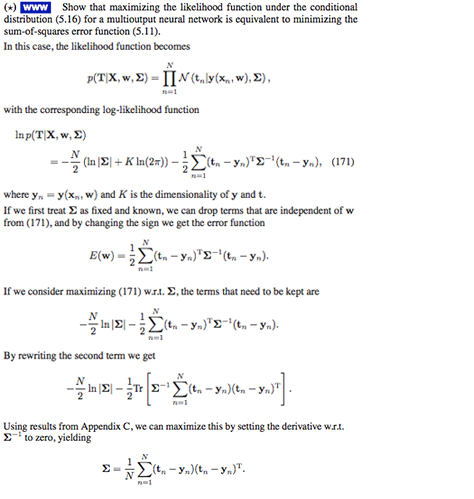
\includegraphics[width=\columnwidth]{images/bishop5-3.png}
        
%         \label{fig:my_labeflf}
%     \end{figure}

% \begin{figure}[H]
%         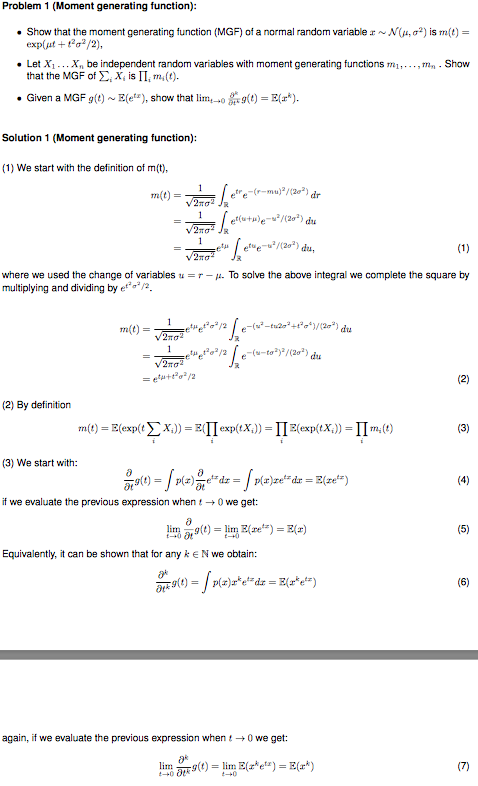
\includegraphics[width=\columnwidth]{images/ex11p1.png}
        
%         \label{fig:my_labelf}
%     \end{figure}


